% !TEX root = catron-dissertation.tex
\epstopdfsetup{outdir=./images/08_conclusion/}

\chapter{Conclusion}
\label{chap:08_conclusion}
\textcolor{red}{
  \begin{itemize}
    \item Please double check my estimate for $\opdrms$ from Stas's paper
  \end{itemize}
}

When an airborne optical system is tested in a wind tunnel, there is a number of sources that contaminate the measurement with noise.
This can be seen if Figure \ref{fig:08_dispersion_isosurface} which shows a multidimensional spectral estimation of an optical wavefront measurement made in a wind tunnel.
\begin{figure}
  \centering
  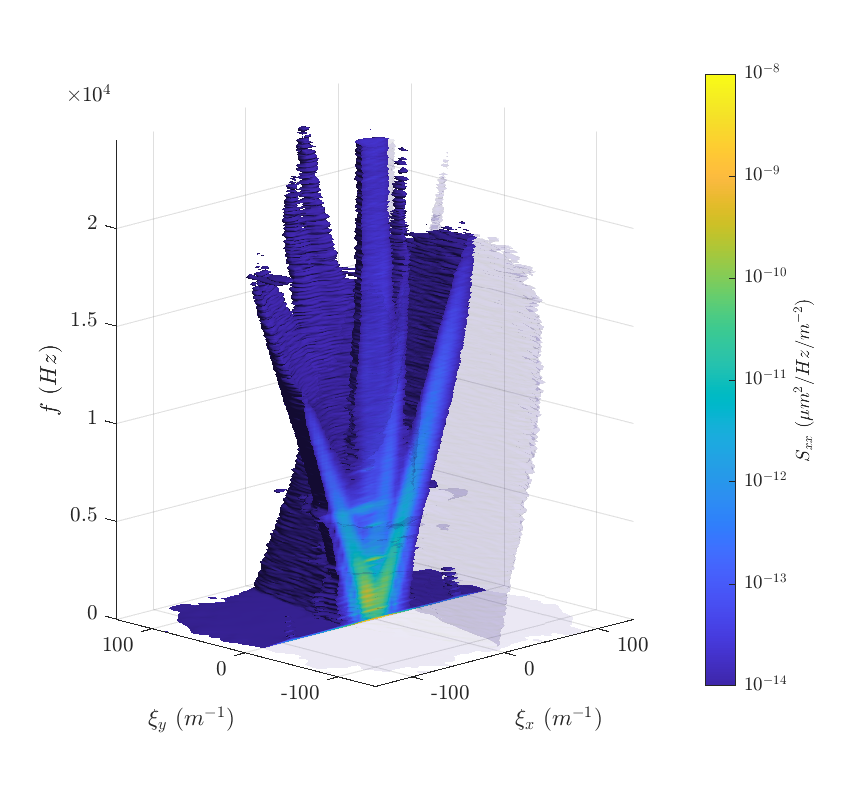
\includegraphics{../matlab/08_conclusion/dispersion_isosurface.eps}
  \put(-195,120){\rotatebox{76}{\Large Boundary Layer}}
  \put(-305,250){\rotatebox{-75}{\Large Acoustic Cone}}
  \put(-300,69){\textcolor{white}{\Large BPF $\Longrightarrow$}}
  \put(-231,180){\textcolor{white}{\rotatebox{90}{\Large Stationary Modes}}}
  \put(-235,50){\rotatebox{15}{\Large Mean-Lensing}}
  \caption{Multidimensional spectral estimation of an optical wavefront measurement made in a wind tunnel.}
  \label{fig:08_dispersion_isosurface}
\end{figure}
The half of the isosurface which represents the portion of the signal that has a component that is traveling vertically downward has been made transparent to show some of the internal power spectrum of planar waves that are traveling parallel to the direction of flow.

In Figure \ref{fig:08_dispersion_isosurface}, the aero-optical signal that is being measured is the boundary layer which resembles a thin ellipsoid which has been rotated up from the $\xi_x-\xi_y$ plane by an amount related to the free-stream velocity.
Acoustic duct modes make up a temporally broadband signal that forms a cone and has a significant portion of the signal that travels upstream.
In the $\xi_x-f$ plane the outer surface of the acoustic cone is limited by the sonic lines at $u\pm c$, while in the $\xi_y-f$ plane the limit is at $\pm c$.
The wind-tunnel fan produces temporally narrow-band acoustic and vibration modes that are able to contaminate the wavefront measurement at the blade-passing frequency (BPF) and its various harmonics.

Sources of noise shown in Figure \ref{fig:08_dispersion_isosurface} not related to the acoustics include stationary modes and mean-lensing.
The stationary modes do not travel in any direction, spatial frequencies are near zero and the signal strength is fairly constant in both time and space.
Due to the temporally white-noise nature of this signal, it is likely not physically relevant and could be optical mode noise from the laser, electronic noise in the camera, or even numerical noise from the processing code.
At lower frequencies, especially around the blade-passing frequency or its harmonics, there is likely be a significant number of stationary modes that are due to vibration of various optical elements.
The mean-lensing portion of the signal ($\lessapprox 100$ Hz) is a slowly varying signal with large spatial-frequency content.
A color coded multidimensional spectral estimation plot that allows for easier identification of the various component signals is shown in Figure \ref{fig:05_synthetic_dispersion_input} and was used for generating a synthetic wavefront.

\section{Filtering of Optical Wavefronts}
Two main families of filtering techniques were examined in this dissertation.
The first family was single sensor filters, Chapter \ref{chap:06_single_filter}, which operate on the optical wavefronts without knowledge of any other time resolved data.
Some of these filters may rely on additional information about the average sampling conditions used to measure the wavefronts.
The second family was multiple sensor filters, Chapter \ref{chap:07_multiple_filter}, which filter the optical wavefront using time resolved measurements from additional sensors.

\subsection{Single Sensor Filters}
The single sensors filters operated directly on the optical wavefront measurements.
Most of these filters are based on Butterworth filters \cite{Butterworth-1930-DvDrjKha} that operate in the multidimensional Fourier domain using a transfer function, $\hat{H}(\xi_x,\xi_y,f)$,
\begin{equation}
  \widehat{WF}(\xi_x,\xi_y,f) = \hat{H}(\xi_x,\xi_y,f)\fftthree(wf(x,y,t)) \textrm{,}
\end{equation}
which can be inverse Fourier transformed back into the physical domain or be used for calculating the multidimensional spectrum.
Filtering can also be performed on the multidimensional spectrum using the gain function, $G^2 = \hat{H}\hat{H}^*$,
\begin{equation}
  S_{xx}(\xi_x,\xi_y,f) = G^2(\xi_x,\xi_y,f)S_{xx}(\xi_x,\xi_y,f) \textrm{.}
\end{equation}
The only filter that was investigated that was not based on basic filters was a baseline spectrum estimator \cite{Schulze-2012-GmyAqzC7}.
This filter removes narrow-band peaks and noise peaks along the temporal-frequency axis smooth spectrum.

Among the filters discussed, three are useful for isolating aero-optical signals from a wavefront.
The first of these is a filter for separating the portion of the optical disturbances that are moving either upstream or downstream realities to the flow (Section  \ref{chap:06_up_down_filter}).
An undesirable effect of this filter is that some signals maybe split if a portion of the signal crosses the separation plane, which can happen to the boundary-layer signal at low temporal-frequencies.
The second useful filter is the low-pass velocity filter which preserves the signal that is moving within a narrow velocity range (Section \ref{chap:06_velocity_filter}).
The third useful is the baseline estimator (Section \ref{chap:06_baseline}), which removes the narrow-band signals associated with the blade-passing frequency and its harmonics, the mean-lensing component, and other temporally narrow-band signals.
Some of these removed narrow-band signals could be relevant signals created by a wind-tunnel model that would be unfortunately removed.

Figure \ref{fig:08_dispersion_filters} shows the multidimensional spectra of the output of these three filters individually plus the spectra of these three filters combined.
\begin{figure}
  \centering
  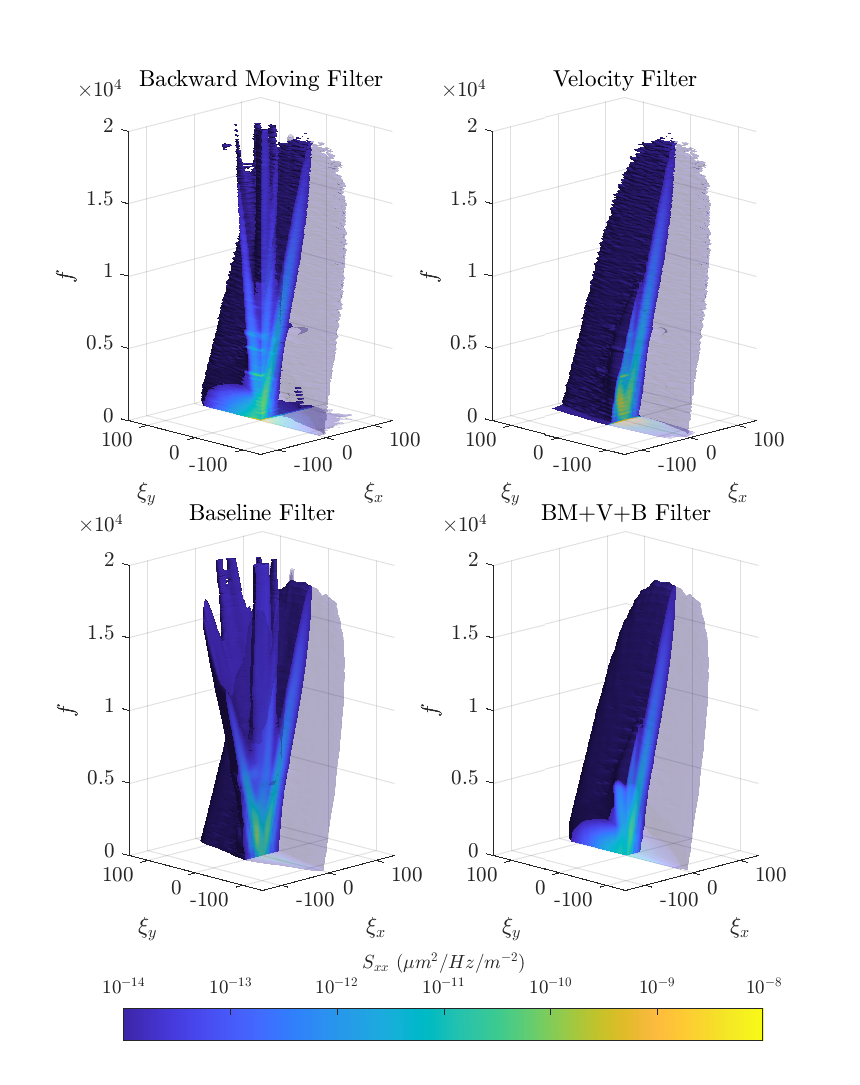
\includegraphics{../matlab/08_conclusion/dispersion_filters.eps}
  \caption{Multidimensional spectra of three single sensor filtering techniques and a combination filter.}
  \label{fig:08_dispersion_filters}
\end{figure}
The forward filter (Figure \ref{fig:08_dispersion_filters} top left) does remove some of the boundary-layer signal at low temporal-frequencies.
The portion of the acoustic cone and stationary modes that are on the downstream-moving portion of the spectrum are retained.
The velocity filter (Figure \ref{fig:08_dispersion_filters} top right) removes most of the broadband signal from the various noise sources.
There is a portion of the acoustic cone and stationary modes that intersect or lay near the boundary-layer signal is slightly attenuated producing a slight hump on the upstream-moving side of the boundary-layer that extends up to about 10 kHz and along the $\xi_y$ axis over the range of about $\pm25\ m^{-1}$.

The baseline filter (Figure \ref{fig:08_dispersion_filters} bottom left) removes all of the temporal narrow-band signals including the mean-lensing portion of the spectra.
The noisy surface of the spectra is removed which does eliminate some the the desired boundary-layer signal.
The combination filter (Figure \ref{fig:08_dispersion_filters} bottom right) applies the velocity and forward filter to the baseline filter.
This filter loses some of the boundary-layer signal due to the noisy surface being smoothed out and the portion that crosses into the upstream-traveling portion of the spectrum.
The portion of the the acoustic cone and stationary modes that is the most contaminating in the velocity filter is removed due to the forward and baseline filter.

A zoomed in slice of the multidimensional spectra is shown in Figure \ref{fig:08_dispersion_filters_slices} for the horizontal moving plane waves.
\begin{figure}
  \centering
  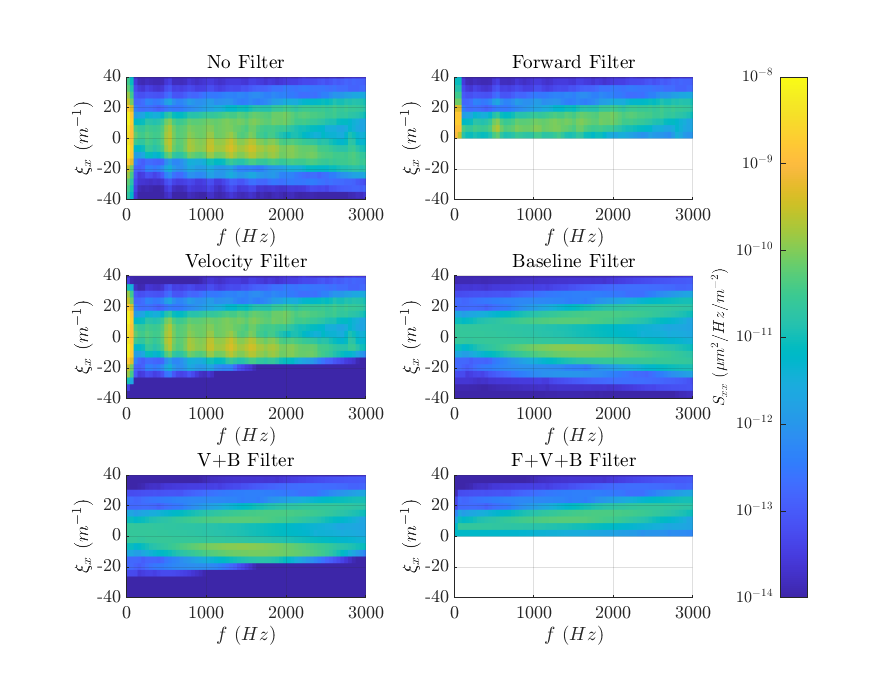
\includegraphics{../matlab/08_conclusion/dispersion_filters_slices.eps}
  \caption{Multidimensional spectral slices for the various single sensor filtering techniques showing the horizontal moving plane waves.}
  \label{fig:08_dispersion_filters_slices}
\end{figure}
A large portion of the single contamination happens at the blade-passing frequency and its harmonics as well as in the mean-lensing region.
This contamination is present in all of the multidimensional spectra that do not utilize the baseline filter.
Even with the velocity filter there is significant contamination on the upstream-moving portion of the spectra due to these narrow-band signals as well as due to the presence of the acoustic cone and stationary modes.
While the forward filter removes some of the boundary-layer signal it removes significantly more of the noise signals that would otherwise be present in the spectra with just the velocity and baseline filters applied.

Representative wavefronts were generated from these multidimensional spectra using the same process as generating a synthetic wavefront from the synthetic spectra in Chapter \ref{chap:05_synthetic} in order to calculate the $\opdrms$.
Table \ref{tab:08_filter_summary} shows the $\opdrms$ values for the various filters used in Figure \ref{fig:08_dispersion_filters_slices}.
\begin{table}
  \centering
  \caption{Summary of single sensor filters}
  \input{../matlab/08_conclusion/dispersion_filters.txt}
  \label{tab:08_filter_summary}
\end{table}
Both the forward and baseline filters reduced the $\opdrms$ of the wavefront a similar amount of 36 and 40\% respectively.
The velocity filter only reduced the $\opdrms$ a small amount of 8.5\% due to the retention of the strongest portion of the narrow-band signals.
The combination of the velocity and baseline filters reduced the $\opdrms$ of the wavefront by 46\% but those still retain a significant portion of the acoustic cone and stationary mode signal.
By combining these three single sensors filters, the $\opdrms$ was reduced 58\% but this is likely under the true value due to some loss of the boundary-layer signal from the forward filter at low temporal-frequencies and the removal of the fluctuations from the baseline filter.
There could be some narrow-band signals that would be generated by a model that would be removed with this filtering scheme.
The estimated $\opdrms$ from Gordeyev \cite{Gordeyev-2014-jcJndkHM} is $0.0112\ \mu m$, which puts the three filter combination in good agreement.

% \begin{figure}
%   \centering
%   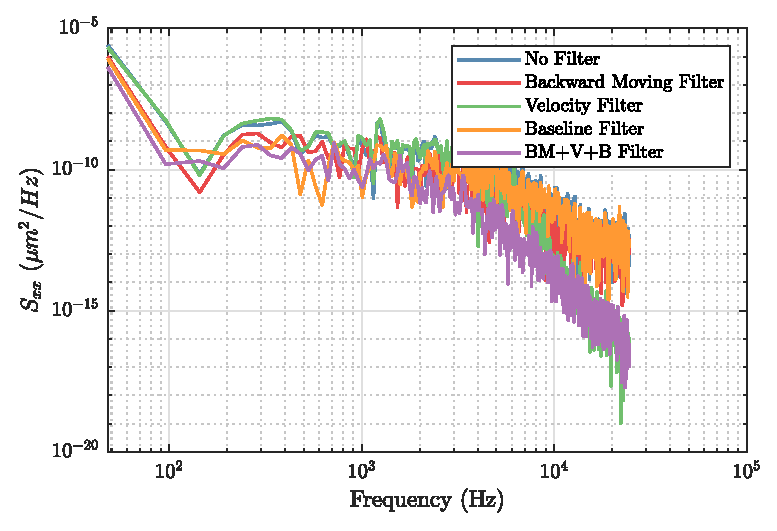
\includegraphics{../matlab/08_conclusion/dispersion_filters_sxx.eps}
%   \caption{Power spectra of the $\opdrms(t)$ for the various single sensor filters.}
%   \label{fig:08_dispersion_filters_sxx}
% \end{figure}

\subsection{Multiple Sensor Filtering}
The multiple sensor filtering used a combination of Linear Stochastic Estimation (LSE) and Spectral Proper Orthogonal Decomposition (SPOD) which has been shown previously to remove vibration noise from wavefront measurements with an approximately 85\% reduction in $\opdrms$ at Mach of 0.3 \cite{DeLucca-2014-RAJvGdv7}.
Similar results were observed using the combination of optical tip/tilt removal and LSE-SPOD on both single dimension (temporal) and multidimensional spectra.
Optical tip/tilt removal alone accounted for a 78.6\% reduction in $\opdrms$, with a combination of 16 microphones and accelerometers and the LSE-SPOD bringing the reduction in $\opdrms$ to 83.9\% at Mach of 0.3.
The combination of tip/tilt removal and the velocity filter showed a greater reduction of 83.9\%.
At a Mach number of 0.5, the use of optical tip/tilt removal, the velocity filter, and 16 sensors in LSE-SPOD, the $\opdrms$ was brought down to 0.0181 $\mu m$ and stilled showed a significant amount of narrow-band signals (see Figure \ref{fig:07_lse_spod} and \ref{fig:07_lse_mspod}).
This is about a 30\% reduction when compared with the other filters used in Table \ref{tab:08_filter_summary}.
This was also significantly above the estimated $\opdrms$ of 0.0112 $\mu m$.

With the LSE-SPOD method the more sensors that were used in the filtering process the greater the reduction in the $\opdrms$, as can be seen in Figure \ref{fig:08_lse_summary}.
\begin{figure}
  \centering
  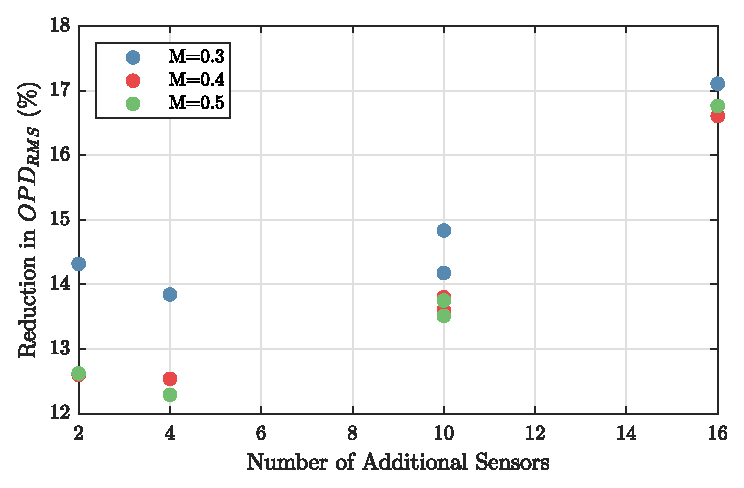
\includegraphics{../matlab/08_conclusion/lse_summary.eps}
  \caption{Percent reduction in $\opdrms$ from the tip/tilt removed case using LSE-SPOD filtering.}
  \label{fig:08_lse_summary}
\end{figure}
With the combination of the DAQ and preamplifier used for the duct mounted microphones they had a fairly low dynamic range possibly leading to the diminished reduction in the four sensor and the lower set at each Mach number of the ten sensor sets.
The signal reduction was fairly uniform with frequency, as shown in Figure \ref{fig:08_lse_mspod_freq}.
\begin{figure}
  \centering
  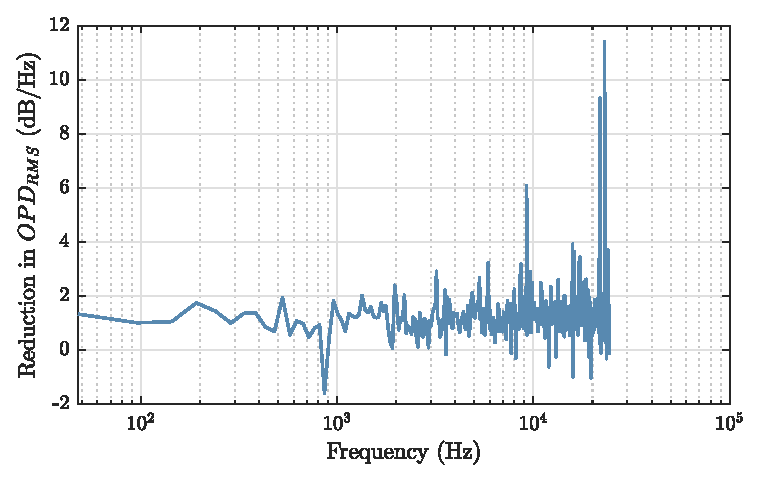
\includegraphics{../matlab/07_multiple_sensor_filtering/lse_mspod_freq.eps}
  \caption{Reduction in $\opdrms$ as a function of temporal-frequency using 16 sensors with LSE-SPOD in the M=0.5 case when compared to tip/tilt removal.}
\end{figure}
On average there was a 1.3dB/Hz reduction in the $\opdrms$ with typically slight peaks at some of the significant narrow-band signals.
At the blade-passing frequency there was a 2dB/Hz reduction and at the narrow-band signals around 3 and 6 kHz there was a 3dB/Hz reduction.
The first, second, and third harmonics of the blade-passing frequency had a below average reduction in the signal.

While the use of additional sensor measurements to aid in filtering of optical wavefront measurements using LSE-SPOD showed little benefit in this study (at least compared to the single sensor filtering techniques), it could show significant benefit in future measurements.
For measurements with models that are likely to create narrow-band signal noise, additional sensor information could utilized in conjunction with a baseline filter for determining which narrow-band signals need to be added back into spectrum.
If at some point in the future there is an algorithm that shows significant benefit in filtering wavefront data with the aid of additional sensor measurements, having the ability to go back into old data and quickly test maybe worth the extra effort in the near term.

\section{Other Useful Products}

\subsection{Synthetic Wavefront}
A synthetic wavefront was developed in Chapter \ref{chap:05_synthetic} to test various filters used in Chapter \ref{chap:06_single_filter}.
In the process used to create the synthetic wavefront, each of these signal components was generated separately in the multidimensional spectrum.
While this synthetic wavefront generation technique produced a qualitative approximation of a wavefront, it provided a useful set of known fully known data to test various filters.
There is some significant room for improvement in the process of creating synthetic wavefront that are more physically accurate.
Even without improvement this process maybe useful in generating a set of synthetic wavefronts with a known aero-optical and noise components that can be used for training a neural network to filter \cite{Lo-1994-W6aWeuaT} wavefront measurements.
A neural network based filter may be able to separate the overlapping component signals at low frequencies.

\subsection{Measuring Acoustic Field Optically}
In section \ref{sect:03_examples_spherical}, optical wavefront were shown to have a fairly good agreement with a microphone for measuring the fluctuating field strength of a spherical wave generated by a speaker.
the optical wavefront measurement however had issues when the acoustic field diverged from being nearly spherical.
Optical wavefronts can make for a excellent way to non-intrusively measure an acoustic field if the field closely resembles a model.

\subsection{Acoustic Mode-Marching}
An acoustic mode-marching method was utilized to quickly estimate the acoustic field within a wind-tunnel test-section assuming that the primary noise source was the wind-tunnel fan.
This is likely to have limited application in filter of optical wavefronts, it maybe useful for assisting in determining whether specific narrow-band signals are likely a product of the wind-tunnel fan and can be filtered out.
There also maybe some application during the initial design of a tunnel for estimating the acoustic field in some critical components.
